\chapter{Literature Review}

This project is centred around the concept of \ac{CL}: the process of acquiring or creating knowledge as part of a group, and the dynamics that emerge when a team needs to manage
participation, the overall success of an activity and the learning objectives that need to be fulfilled \parencite{laal_2012}. It is also possible to analyse the concept as
learning to collaborate, to acquire the skills needed to be an effective team member.

The purpose of this literature review is to find the benefits of adopting a \ac{CL} approach in a learning design and the challenges that any educator needs to consider when
implementing a strong focus on collaboration. It is also important to understand why collaboration and teamwork are such important skills to develop, why is it so valued in
most professional environments and why is there a general feeling that educative institutions are failing in teaching those skills.

This research will approach the field of \ac{CL} using the lens of \ac{TEL}: the use of technologies to support processes or management of teaching and learning \parencite{passey_2019}.
Understandably, this is still too wide of a subject, so, a particular focus is set on \ac{AR} technologies. The objective will be to understand how \ac{AR} can be used in the classroom,
and the particularities that it offers in terms of benefits, challenges, common implementations and relevant success stories.

\ac{AR} can be a valuable collaborative learning tool based on the unique abilities it possesses. Specifically, the technology excels at incorporating strong visuals into the surroundings
of the user(s), which provides an opportunity to design enticing experiences for both learning and collaboration. For this purpose, it is important to identify what collaborative
experiences have been created in the past with \ac{AR}, what learning goals align with the technology and what challenges in design and development can be expected.

This chapter explores these questions and themes across three sections. The first section tackles the topic of collaboration, how it is defined and measured, different implementations in
the classroom, perceived benefits, common challenges and lessons learned from previous projects. The second section presents a systematic literature review aimed at identifying the use of
\ac{AR} as a tool for education, how the technology has evolved, which elements of the technology have derived in success stories, and which have become challenges. The final section will
combine both subjects and explore the literature for previous experiences using collaborative \ac{AR}, both in education and in other fields.

\section{Collaborative Learning}
\subsection{Collaboration as a Transversal Skill}

The subject of \ac{CL} is wide and can be tackled through different angles. For instance, we can talk about collaboration as an isolated term, and relate it to similar concepts like teamwork,
cooperation and intrapersonal skills. In need of a definition, the approach taken by \textcite{andriessen_2020} is very complete. The authors state that ``(…) collaboration means developing, in
an equal and mutually respectful way, a shared view of a situation”. Is a simple definition that implies two important things. First, collaborators find themselves in equal terms, there is a
sense of equality and mutual correspondence. Authoritative or hierarchical relations hardly produce collaborative settings. Second, collaboration goes beyond cooperation, beyond working together
to fulfil a goal. Collaboration implies building, through time, a shared view. The group has a shared set of goals, purpose and values. The classical definition of collaboration proposed by
\textcite{omalley_1995} also complements this idea by stating that cooperation involves the division of labour among participants, of individual responsibility, while collaboration is a
coordinated effort to solve the problem. Echoing this distinction between collaboration and similar ideas like cooperation or teamwork, \textcite{salmons_2019} states that collaboration is a
process that needs to constantly be managed, while teamwork is a more \emph{natural} or \emph{improvised} way of working together when needed.

\textcite{andriessen_2020} later expand all these ideas by stating how collaboration is built through time in three different dimensions. In a personal sense, we collaborate because we gain
something from it, or in the worst-case scenario, because we need to do it. Our goals align with those of others, creating a second inter-personal dimension, in which we also care about the
relationship we create with others and the social advantages we obtain from the collaboration. Finally, with strong inter-personal interactions, we create a group dynamic, in which decisions
are taken beyond the individual level and align with the necessities of the group. This evolution can be fractal, which means that after a strong group has been created, it can be developed
in a fourth dimension, an inter-group relationship in which several tight-knitted groups collaborate in a shared purpose within a bigger system.

Now is possible to build an initial definition to be use as conceptual backbone. Collaboration will be understood as: the process in which a group of people build a set of values, shared views
and coordinated efforts to fulfil a purpose or reach a goal. This definition considers the most important aspects highlighted previously by other authors: collaboration goes beyond just
coordinating tasks because is strongly linked to building relationships and communities, therefore, it is a very social skill. Collaboration is not a single action, is a process that needs time
and effort to be constructed. Finally, collaboration is aimed, it needs a purpose or a goal. More important, that goal needs to be shared among the collaborators instead of being imposed.
Collaboration can only be developed when all the members of the group find themselves as equals and share the perceived value or the necessity of working towards that aim.

It is possible to add more elements to the definition, creating a wider and stronger framework, if we analyse the concept of collaboration from other perspectives and in different contexts. For
instance, collaboration can be viewed as a skill to be developed within the context of professional development and employability.

As stated by \textcite{crant_2000}, it is common for a workspace to seek in a professional a proper balance between theory and knowledge, that is, the information gathered through practice and
experience. This position can be read as employers seeking people that have built a career rather than only have a profession. For employees, it means that they must build that career identity:
the right set of skills, experience and personal traits that show value beyond a profession. Additionally, employers seek candidates that can properly response to a variable environment, either
due to high pressure or a fast-moving market. Employees must then demonstrate personal adaptability, a willingness to explore, and life-long learning values. Finally, employers seek for the ability
to properly construct and use the surrounding social context, the employee needs to build social capital by cultivating abilities in cooperation, networking and teamwork.

This framework shows the importance on adding value to the professional profile, and highlights skills related to adaptability and collaboration as key value pointers. The framework also relates
easily to other popular concepts like social intelligence, personal development and problem-solving attitudes, all part of what has been known as transversal skills. The UNESCO defines transversal
skills as those that can be used in a wide variety of situations and work settings \parencite{unesco_2014} and are valuable for their general applicability and transferability. These skills can be
organized in five broad categories:

\begin{itemize}
    \item Critical and innovative thinking.
    \item Interpersonal skills.
    \item Intrapersonal skills.
    \item Global citizenship.
    \item Media and information literacy.
\end{itemize}

To understand better the type of abilities that the previous categories encompass, we can extract some ideas from diverse sources in the literature, a set of studies focused in understanding the work market
in different contextual variations of geography, professional field, years of experience and even nature of the job-hunting process \parencite{smaldone_2022,ng_2021,nadarajah_2021,boahin_2013,llorens_2017,huynh_2024,zhang_2024,garst_2019,abir_2024}.
This sample of literature shows the type of skills most demanded by employers around the world. Although skills that are considered \emph{hard}, or better described as field-specific are understandably
diverse, there is almost a complete coordination related to \emph{soft}, transversal skills. These skills are common to all contexts and independent of the region or work field. Figure \ref{fig:2-1} shows a visual
distribution of the most common transversal skills sough after in potential candidates, extracted from the studies mentioned above.

\begin{figure}[t]
    \centering{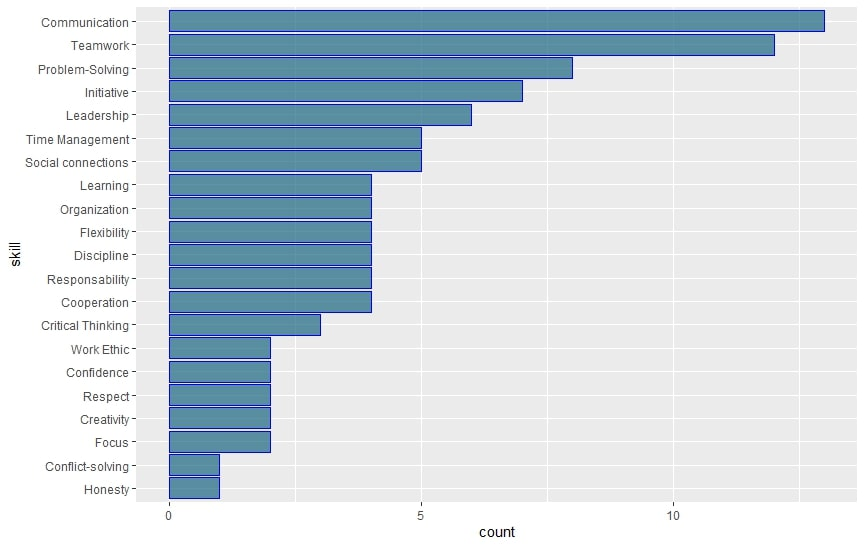
\includegraphics[alt={Figure 2.1},width=0.99\textwidth]{figures/F2-1.jpg}}
    \caption{Most common soft skills identified \label{fig:2-1}}
\end{figure}

Despite being a small sample, the data shows a clear emphasis on relational skills, and it seems to portray the added value of hiring and developing people with high communication abilities, teamwork, good
social interactions, and flexibility \parencite{al-asefer_2021}.

Another important sentiment that can be extracted from all the literature mentioned is a perceived discordance between the skills and abilities focused on by high educational organisations and those sought
after by companies and employees, as identified so far in this section \parencite{ng_2021,damoah_2021}.

\textcite{tulgan_2023} identifies specifically three soft skills missing in young workers: professionalism, critical thinking and teamwork. Tulgan argues that this gap is closely related to a generational
and technological shift where there is a lower need to develop communication skills because we have offloaded most of our communicational needs into electronical devices (mails, meetings, conversation, social
interactions), forgoing the opportunity to develop such skills in person.

Tulgan keeps explaining that in recent years \emph{good old-fashioned} teamwork became an issue for young people, who have developed a different set of values that clash with those of previous generations. Where
older generations built a long career as part of a company or institution, newer generations have little to no loyalty to a single employer, and they are more likely to search for better deals. Young professionals
find little value in adapting to the ways and stablished institutions of a group when they know very well, they won't be there for too long.

Secondary and tertiary education programs are often seen as the main responsible agents in the development of skills deemed crucial for the general professional life \parencite{kechagias_2011} and is in this light
that modern curricula in almost all disciplines now have a higher emphasis on building those transferable skills \parencite{dhir_2021}. This is not without problems, and there is a noticeable consensus that teaching
such skills is not a trivial task \parencite{mccale_2008}. Several factors influence the ability of a curriculum to provide such learning pathways. Most common problems are related to how little educators are prepared
to incorporate those skills in their classrooms \parencite{kemp_1995}, the costs of adapting the curriculum, training the personnel and changing old mindsets to effectively provide the space to create such learning \parencite{chadha_2006}.

Considering these extra contextual elements, it is possible to modify the previous definition of collaboration as follows: Collaboration is the skill to work as part of a group by identifying, building and acting upon
a set of values, shared views and coordinated efforts to fulfil a purpose or reach a goal. This modified definition not only states a set of characteristics of what the process of collaborating implies, it frames it as
a skill to be executed by each member of a group, and not as something that happens naturally when people gather. It also acknowledges the need to learn and develop such skills.

The theoretical framework around collaborative learning can be expanded by exploring the definition of a second concept, that of Communities of Practice, with the intention of later linking this idea with the general
definition of collaboration built so far and the approach proposed by this project to use it as an educational tool.

\subsection{Communities of Practice}

A term proposed by \textcite{lave_1991}, a \ac{CoP} can be defined as a set of mechanisms of situated learning used by communities to transmit knowledge internally, especially to newer members. These communities are
formed around a focused domain and were initially used to describe the learning process used in different trades like craftmanship and health practices. The meaning of the term has been broadening with time and can
be applicable to any group that gathers towards a common goal over an extended period, that is, enough time for several generations of members to come and go.

Strongly linked to \ac{CoP} is the idea of legitimate peripheral participation. This can be defined as the process in which newcomers learn mostly through observation and gradual participation with their senior peers \parencite{mcdonald_2017}.
\ac{CoP} are used to give some structure to the process of informal learning, especially the type of learning found outside of academy, and which is more linked to professional practice, personal development and the
relationships forged in the day-to-day activities with peers and a community in general.

A healthy \ac{CoP} is one that is generated naturally due to the interaction of a community around a specific domain. It is different from a task force or team of people gathered around a goal or a problem in the
sense that the general objective of a \ac{CoP} is more undefined in terms of time, is focused more on the practice rather than the goal or product itself and is constituted by a social community rather than by just
a collaborating team of people. These are the three fundamental elements that define a \ac{CoP}: a domain, a community and a stablished practice, as described in Figure \ref{fig:2-2}.

\begin{figure}[t]
    \centering{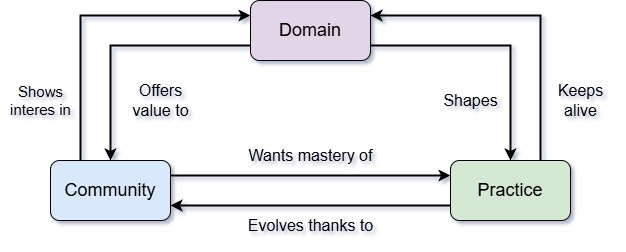
\includegraphics[alt={Figure 2.2},width=0.99\textwidth]{figures/F2-2.jpg}}
    \caption{Elements of a Community of Practice \label{fig:2-2}}
\end{figure}

The domain is the knowledge base in which the community chooses to work because it offers value or just interest in general. New members come voluntarily and interact with elder members gaining experience in the practice,
with the expectation of eventually gaining mastery.

The community is a group of people that can be driven by complex social dynamics. The community will create norms, stratifications and behaviours over time. The community is expected to be in a constant flux of members and
to evolve with time, in terms of social interactions and the relationship it has with the domain.

The practice is an integrated set of activities and knowledge executed and transmitted by the community to create mastery over them. Some \ac{CoP} focus more on nurturing members into the mastery of the practice, while other
focus more on the transmission and preservation of the knowledge generated, as noted by \textcite{klein_2005}.

\ac{CoP} have shown to be the cornerstones in the development of informal and social learning, leadership development and organizational change \parencite{anderson_2013}. Often, high indexes of performance and employee
satisfaction are present when a \ac{CoP} has been identified and nurtured within the informal structure of an organization \parencite{blackmore_2010}. Also, they have proven to be valuable integration, communication, and
identity reinforcement tools in communities with a high degree of disparity or diversity among members \parencite{hildreth_2004}.

A particular emphasis in the idea of nurturing a \ac{CoP} is important. A community can perish due to lack of proper nourishment or caused by artificial intervention. Previously it was noted that it is not possible to force the
creation of a \ac{CoP}, new members must voluntarily engage in legitimate ways with the practice. But even when a community develops and grows in members, and its value is acknowledged and sough after, forced practices that run
in contradiction with the spirit of a \ac{CoP} can end up killing it. Authors like \textcite{ardichvili_2003} and \textcite{brown_1991} have analysed the lifecycles of successful and failed \ac{CoP} inside the organizational
practice of many and varied industries, from insurance brokers to high education institutes. Of all the key factors identified in the failure or disappearance of a \ac{CoP}, it is useful to highlight the following ones:

\begin{itemize}
    \item Not allowing enough time for members of the community to form relationships and sustain them. This can be due to frequent administrative reorganization or the prevalence of temporary or part-time staff.
    \item A culture of tight management, where every aspect of the practice is highly standardized and supervised, and there is no possibility for a natural development of the practice due to the relationships formed in the community.
    \item A culture of highly individualized work, either due to the very nature of the practice or because of other factors, like a very competitive environment. This inhibits collaboration and discourages collective engagement.
    \item Practices with extreme time or performance pressures, which leaves little time to develop a collective or communicative environment.
    \item Spatially fragmented work, so that there is no opportunity to establish a relationship, or because there is not a common, unsupervised space for the community to gather.
    \item Communication and activities are heavily mediated by technology or even other people. This makes interactions (arguably) less immediate and intense, therefore, lacking importance.
\end{itemize}

So far, all the elements that have been illustrated paint the concept of a \ac{CoP} as a natural-occurring social structure formed around the need of preserving, communicating and nourishing knowledge within a well stablished community.
It is a manifestation of informal education that thrives and offers the best results when acknowledged at an organizational level but not tampered with \parencite{brown_1991}, and when given enough resources to grow and evolve \parencite{klein_2008}.

Given the importance of naturality and informality within the definition of a \ac{CoP}, it is possible to see how these fundamental elements can be at odds with the expectations and common practices found in more traditional and
institutionalized education, where learning is more structured, participation is hardly voluntary and collaborative processes are more task-focused rather than long-term approaches to the practice. These issues will be acknowledged in the
following section.

\subsection{Communities of Practice and Education}